\documentclass[journal,12pt,twocolumn]{IEEEtran}

\makeatletter
\makeatother
\usepackage{setspace}
\usepackage{gensymb}
\usepackage{xcolor}
\usepackage{caption}

\singlespacing

%\usepackage{geometry}
%\geometry{letterpaper}

\usepackage{graphicx}
\graphicspath{ {./images}  }
\usepackage[cmex10]{amsmath}
\usepackage{mathtools}
\usepackage{wasysym}
\usepackage{amsthm}
\usepackage{mathrsfs}
\usepackage{txfonts}
\usepackage{stfloats}
\usepackage{cite}
\usepackage{cases}
\usepackage{mathtools}
\usepackage{subfig}
\usepackage{enumerate}	
\usepackage{enumitem}
\usepackage{amsmath}

\usepackage{longtable}
\usepackage{multirow}

\usepackage{enumitem}
\usepackage{mathtools}

\usepackage{listings}
\usepackage{listings}
\usepackage[latin1]{inputenc}                                
\usepackage{color}                                            
\usepackage{array}                                            
\usepackage{longtable}                                        
\usepackage{calc}                                             
\usepackage{multirow}                                        
\usepackage{hhline}                                          
\usepackage{ifthen}    
\usepackage{lscape}

\DeclareMathOperator*{\Res}{Res}
\renewcommand\thesection{\arabic{section}}
\renewcommand\thesubsection{\thesection.\arabic{subsection}}
\renewcommand\thesubsubsection{\thesubsection.\arabic{subsubsection}}
\hyphenation{op-tical net-works semi-conduc-tor}
\def\inputGnumericTable{}                            

\lstset{
%language=python,
frame=single, 
breaklines=true,
columns=fullflexible
}

%\usepackage{amssymb}
%\usepackage{epstopdf}
%\title{Brief Article}
%\author {The Author}

\begin{document}
%\maketitle

\theoremstyle{definition}
\newtheorem{theorem}{Theorem}[section]
\newtheorem{problem}{Problem}
\newtheorem{proposition}{Proposition}[section]
\newtheorem{lemma}{Lemma}[section]
\newtheorem{corollary}[theorem]{Corollary}
\newtheorem{example}{Example}[section]
\newtheorem{definition}{Definition}[section]

\newcommand{\BEQA}{\begin{eqnarray}}
\newcommand{\EEQA}{\end{eqnarray}}
\newcommand{\define}{\stackrel{\triangle}{=}}

\bibliographystyle{IEEEtran}

\providecommand{\nCr}[2]{\,^{#1}C_{#2}} % nCr
\providecommand{\nPr}[2]{\,^{#1}P_{#2}} % nPr
\providecommand{\mbf}{\mathbf}
\providecommand{\pr}[1]{\ensuremath{\Pr\left(#1\right)}}
\providecommand{\qfunc}[1]{\ensuremath{Q\left(#1\right)}}
\providecommand{\sbrak}[1]{\ensuremath{{}\left[#1\right]}}
\providecommand{\lsbrak}[1]{\ensuremath{{}\left[#1\right.}}
\providecommand{\rsbrak}[1]{\ensuremath{{}\left.#1\right]}}
\providecommand{\brak}[1]{\ensuremath{\left(#1\right)}}
\providecommand{\lbrak}[1]{\ensuremath{\left(#1\right.}}
\providecommand{\rbrak}[1]{\ensuremath{\left.#1\right)}}
\providecommand{\cbrak}[1]{\ensuremath{\left\{#1\right\}}}
\providecommand{\lcbrak}[1]{\ensuremath{\left\{#1\right.}}
\providecommand{\rcbrak}[1]{\ensuremath{\left.#1\right\}}}
\theoremstyle{remark}
\newtheorem{rem}{Remark}
\newcommand{\sgn}{\mathop{\mathrm{sgn}}}
\providecommand{\abs}[1]{\left\vert#1\right\vert}
\providecommand{\res}[1]{\Res\displaylimits_{#1}} 
\providecommand{\norm}[1]{\lVert#1\rVert}
\providecommand{\mtx}[1]{\mathbf{#1}}
\providecommand{\mean}[1]{E\left[ #1 \right]}
\providecommand{\fourier}{\overset{\mathcal{F}}{ \rightleftharpoons}}
\providecommand{\system}{\overset{\mathcal{H}}{ \longleftrightarrow}}

\newcommand{\solution}{\noindent \textbf{Solution: }}
\providecommand{\dec}[2]{\ensuremath{\overset{#1}{\underset{#2}{\gtrless}}}}
\DeclarePairedDelimiter{\ceil}{\lceil}{\rceil}
\numberwithin{equation}{section}

\let\StandardTheFigure\thefigure
\let\StandardTheFigure\thefigure
\let\StandardTheTable\thetable

\def\putbox#1#2#3{\makebox[0in][l]{\makebox[#1][l]{}\raisebox{\baselineskip}[0in][0in]{\raisebox{#2}[0in][0in]{#3}}}}
     \def\rightbox#1{\makebox[0in][r]{#1}}
     \def\centbox#1{\makebox[0in]{#1}}
     \def\topbox#1{\raisebox{-\baselineskip}[0in][0in]{#1}}
     \def\midbox#1{\raisebox{-0.5\baselineskip}[0in][0in]{#1}}
     
 \title{ Principal Component Analysis}
 
 \author{Nisha Akole, G V V 
Sharma$^{*}$% <-this % stops a space
\thanks{*The authors are with the Department
of Electrical Engineering, Indian Institute of Technology, Hyderabad
502285 India e-mail:  gadepall@iith.ac.in.}
}
\maketitle

\tableofcontents

\bigskip

\begin{abstract}
%\boldmath
This manual provides a brief description on how to implement Principal Component Analysis from scratch and use it for dimensionality reduction of data.
\end{abstract}

\IEEEpeerreviewmaketitle

\section{Objective}
Our objective is to implement PCA and reduce dimensionality of data which gives better understanding of data visually.

\section{Load Dataset}
The dataset used for PCA is available at the following link. Download all the data file in the folder where you want to write code for PCA.
\begin{lstlisting}
https://github.com/prabhatrai111/Commensal-Radar
\end{lstlisting}
\begin{lstlisting}
import numpy as np
import scipy.io as sio
from sklearn.utils.extmath import randomized_svd

mat_contents = sio.loadmat('data_all.mat')
X_data = mat_contents['data_all']
\end{lstlisting}

\section{About PCA}
Principal component analysis (PCA) is a statistical procedure that uses an orthogonal transformation to convert a set of observations of possibly correlated variables (entitles each of which takes on various numerical values) into a set of values of linearly uncorrelated variables called principal components.
There are four main operations in the PCA:\\
		1) Pre-processing\\
		2) Co-variance Matrix\\
		3) Eigen Vectors\\
		4) Feature Vector and Plot

\section{Pre-processing}
Take the whole dataset ignoring the labels. Feature scaling is an important task in PCA because various scales of feature will affect and we may not get an optimized output. The functions  StandardScaler or MinMaxScaler will standardize the features by making mean $=0$ and variance $=1$. These functions are imported from sklearn.preprocessing. 
StandardScaler uses formula such as 
$$ z = (X-\mu)/\sigma$$
where, $\mu = $Mean of data X\\
$\sigma =$Standard Deviation of data X\\

\begin{lstlisting}[mathescape=true]
X = np.matrix(X_data)
$\mu = X.mean(0)$
$\sigma =X.std(0)$
X_std$ = (X-\mu)/\sigma$
\end{lstlisting}

X.mean(0) and X.std(0) will give columnwise mean and standard deviation of our data matrix.

\section{Compute Covariance Matrix}
Computing the covariance matrix will help us to understand the relationship between the variables. If variables are highly correlated, they contain redundant information. Covariance matrix will be symmetric with diagonal values as a variance of the corresponding element. If variables are increasing or decreasing together, then its positive covariance.If one variable is increasing and other is decreasing, sign of covariance will be negative.
 
\begin{lstlisting}[mathescape=true]
X_cov = np.cov(X_std)
\end{lstlisting}

\section{Compute Eigenvectors}
The diagonal values of covariance matrix are the eigenvalues of a covariance matrix where large eigenvalues correspond to large variance. Eigenvector of covariance matrix is the axes along with data has maximum variation. Eigenvalues and eigevectors can be calculated by taking Singular Value Decomposition(SVD) of a covariance matrix. Eigenvalues are arranged in decreasing order in sigma matrix and its corresponding eigenvector is arranged in U which is left eigenvector or eigenvector of np.matmul(X\_cov,X\_cov'), where X\_cov' is transpose of X\_cov.
\begin{lstlisting}[mathescape=true]
U, $\Sigma$, VT = randomized_svd(X_cov, n_components=10 ,n_iter= 5, random_state=none)
\end{lstlisting}
n\_components will consider first 10 largest eigenvalues. Hence, first 10 eigenvectors will be used for plotting the data and these eigenvectors are known as principal components which carries maximum information.

\section{Principal Component and plot}
To visualize the data either we can plot it in 2D or 3D. But sometime first 2 or 3 principal components are not sufficient to retain the maximum information from dataset. In such case, no of principal components can be decided by taking ratio of first K eigenvalues to sum of all the eigenvalues. If the ratio is closer to 0.95 then these K principal components are taken. Link for PCA without function is given below:
\begin{lstlisting}[mathescape=true]
https://github.com/NishaAkole/AI-and-ML/blob/master/codes/pca/PCAwithoutFun.py
\end{lstlisting}
  
The above whole program can be combined except preprocessing and a single command(i.e using inbuilt function) can do all the  
\begin{lstlisting}[mathescape=true]
https://github.com/NishaAkole/AI-and-ML/blob/master/codes/pca/PCAFun.py
\end{lstlisting}

\section{Figures}
\begin{figure}[!h]
\begin{center}
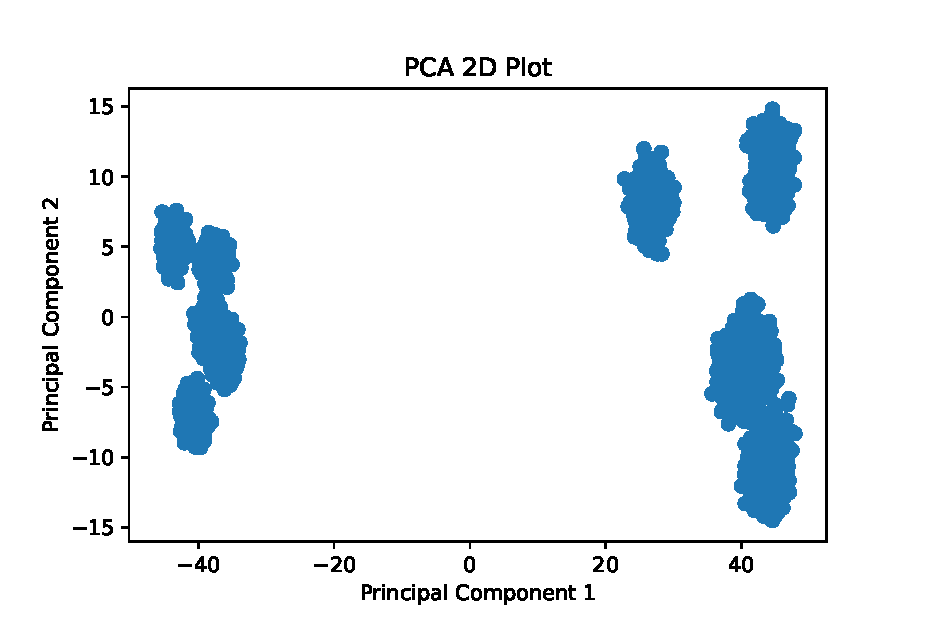
\includegraphics[width=3in]{./figs/PCA_2D.eps}
\end{center}
\caption{PCA with Function 2D}
\label{fig: 2D Plot}
\end{figure}

\begin{figure}[!h]
\begin{center}
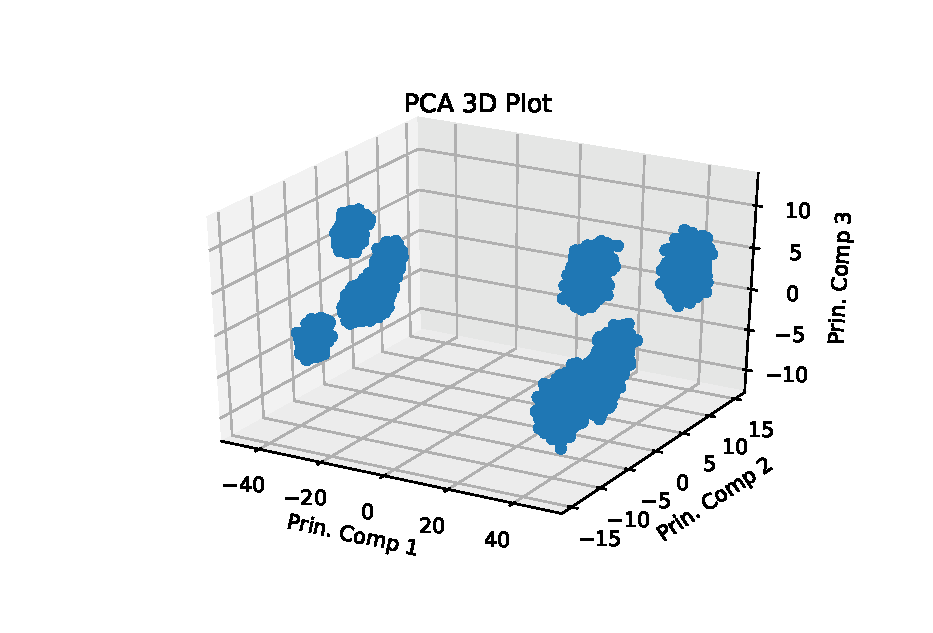
\includegraphics[width=3.8in]{./figs/PCA_3D.eps}
\end{center}
\caption{PCA with Function 3D}
\label{fig: 3D Plot}
\end{figure}

\begin{figure}[!h]
\begin{center}
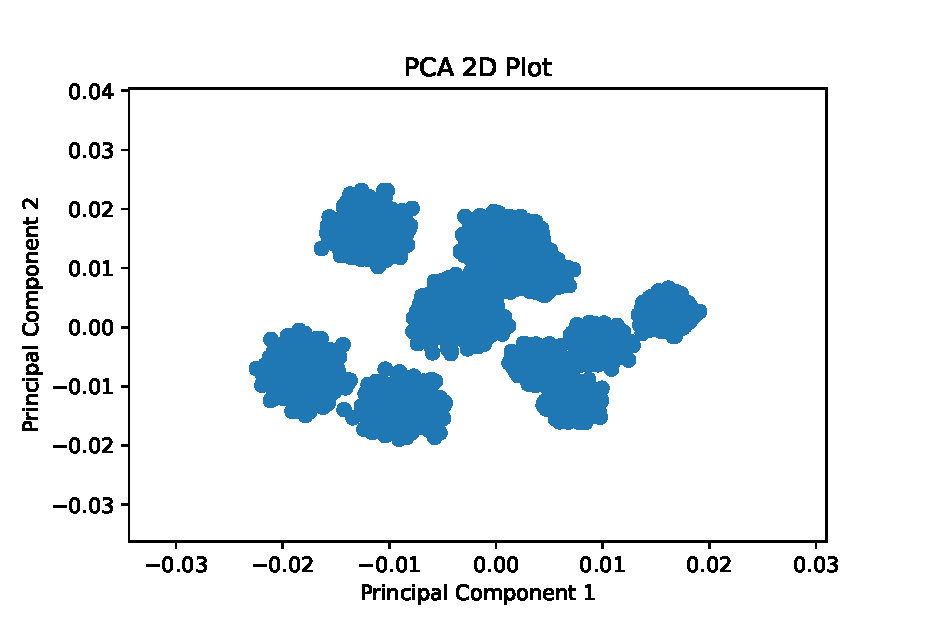
\includegraphics[width=3in]{./figs/PCA_2D_woFun.eps}
\end{center}
\caption{PCA without Function 2D}
\label{fig: 2D Plot}
\end{figure}

\begin{figure}[!h]
\begin{center}
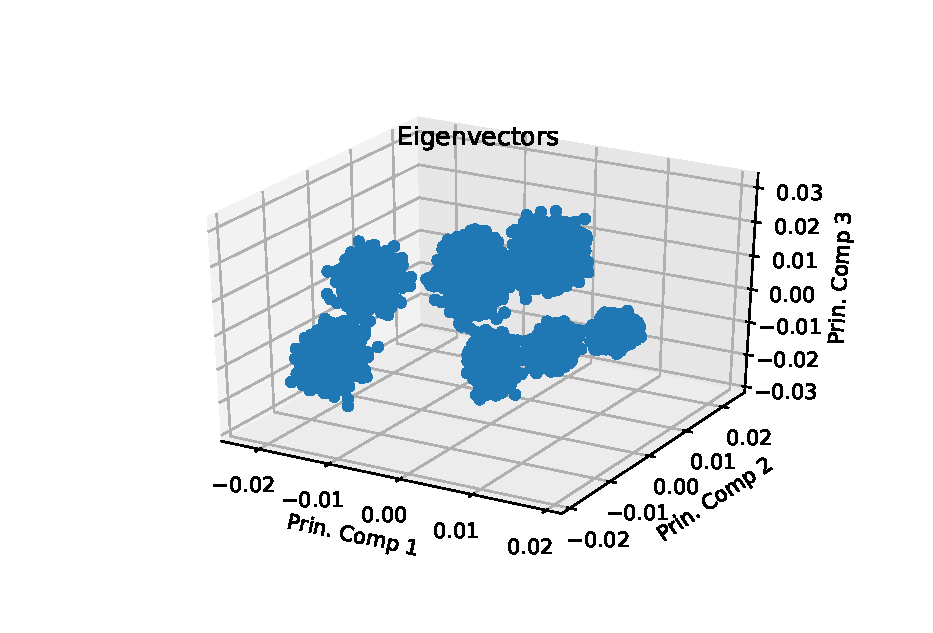
\includegraphics[width=3.8in]{./figs/PCA_3D_woFun.eps}
\end{center}
\caption{PCA without Function 3D}
\label{fig: 3D Plot}
\end{figure}

Above plots help us to visualize the data. To get more idea on principal component and and amount of information it contain through plot below:

\begin{figure}[!h]
\begin{center}
\includegraphics[width=3.8in]{./figs/Accuray.eps}
\end{center}
\caption{Information vs No of Dimensions }
\label{fig: }
\end{figure}  

Clearly, only two or three prin. comp does not contain much info. Hence, PCA is not a good approach for dimensionality reduction for this data.

\end{document}

© 2019 GitHub, Inc.
Terms
Privacy
Security
Status
Help
Contact GitHub
Pricing
API
Training
Blog
About
